\section{Strumenti}
\label{strumenti}
In questa sezione verranno presentati tutti gli strumenti che il gruppo \authorName{} utilizzerà per svolgere le varie attività che compongono i processi. Per ogni strumento verranno esplicate le principali procedure di interazione. Le procedure di installazione si riferiscono ad \textbf{Ubuntu 12.04 LTS}.

\subsection{Strumenti a supporto del processo di sviluppo}

\subsubsection{Git}
\label{git}
\textbf{Git} è un sistema per il controllo di versione di un filesystem. Verrà adottato per ospitare i file del progetto sottoposti a controllo di versione.\\
Versione utilizzata: \textbf{1.8.3.2}

\paragraph{\underline{Installazione}:} per l'installazione dell'applicativo, seguire la seguente procedura:
\begin{itemize}
\item Aprire il terminale;
\item Digitare \verb!sudo apt-get install git-core!;
\item Seguire la procedura di installazione fino al termine.
\end{itemize}

\paragraph{\underline{Best Practise di interazione}:} per evitare conflitti nel repository\g{}, è indispensabile eseguire le seguenti operazioni di sincronizzazione all'inizio e alla fine di ogni sessione di lavoro (fig \ref{usorepo}):
\begin{enumerate}
\item \textbf{Pull:} prima di iniziare la sessione di lavoro, per ottenere i file aggiornati;
\item \textbf{Commit:} al termine di una sessione di lavoro, per commentare le modifiche effettuate;
\item \textbf{Pull:} subito prima di eseguire l'operazione di push;
\item \textbf{Push:} subito dopo l'operazione di pull, per caricare le modifiche nel repository\glossario{} remoto;
\item \textbf{Merge:} se durante l'operazione di push sorgono dei conflitti a seguito di modifiche effettuate da un altro membro.
\end{enumerate}
\begin{figure}[!h]
	\centering
	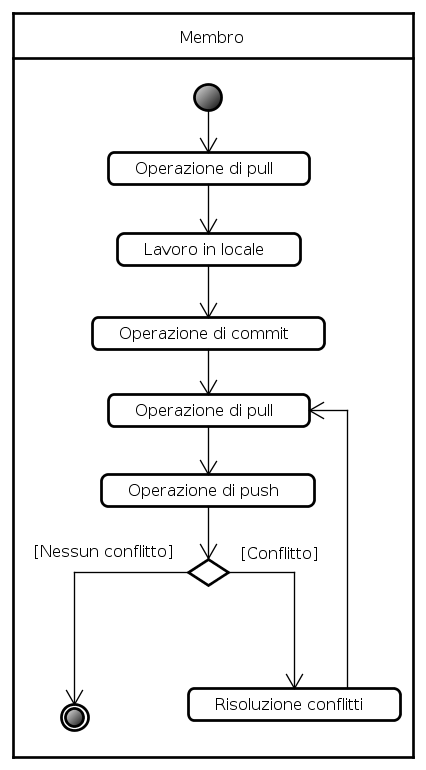
\includegraphics[scale=0.5]{./content/Immagini/Utilizzo_Repository.png}
	\caption{Procedura per l'utilizzo del Repository}
	\label{usorepo}
\end{figure}
I commenti aggiunti al commit dopo la modifica di un file devono essere chiari e devono specificare le modifiche effettuate. Per garantire una buona leggibilità dei commenti, i commit devono essere effettuati per ogni file modificato o gruppo di files dello stesso contesto. Inoltre, per evitare conflitti, è sconsigliato lavorare contemporaneamente sugli stessi file.

\subsubsection{VMware}
\label{vmware}
Software che permette l'emulazione di un determinato sistema operativo. Gli \textit{Amministratori} hanno creato un ambiente, basato su \textbf{Ubuntu 12.04 LTS}, comprendente tutti gli strumenti necessari allo sviluppo del software. Per usufruire di questo ambiente, è però necessario possedere \textbf{VMware Player}.\\
Versione utilizzata: \textbf{6.0.1}

\paragraph{\underline{Installazione}:} per installare il software, seguire la seguente procedura:
\begin{itemize}
\item Collegarsi al sito internet: \url{https://my.vmware.com/web/vmware/free#desktop_end_user_computing/vmware_player/6_0}
\item Selezionare \textit{Download} in corrispondenza del sistema operativo presente nella propria postazione di lavoro;
\item Aprire il terminale;
\item Digitare \verb!sudo apt-get install build-essential linux-headers-$(uname -r)! e procedere con l'installazione;
\item Posizionarsi nella directory contenente il file precedentemente scaricato;
\item Digitare \verb!gksudo bash nome_del_file.bundle! e seguire la procedura di installazione.
\end{itemize}

\subsection{Strumenti a supporto del processo di documentazione}

\subsubsection{Astah}
\label{astah}
\textbf{Astah} è uno strumento multipiattaforma che permette di disegnare svariate tipologie di grafici secondo lo standard UML2.0\g{}.\\
Versione utilizzata: \textbf{6.7.0/43495 Professional Edition}

\paragraph{\underline{Installazione}:} per l'installazione della versione \textbf{Professional} di questo applicativo, è necessario ottenere una licenza per studenti universitari. Seguire la seguente procedura:
\begin{itemize}
\item Collegarsi all'indirizzo \url{http://astah.net/download}
\item Selezionare \textit{Download Free Student Edition}. Verrà caricata una pagina contenente una form;
\item Compilare la form con i propri dati;
\item Selezionare \textit{Send Request}. Verrà inviata una e-mail all'indirizzo indicato e verrà caricata una pagina di ringraziamento;
\item Selezionare il proprio sistema operativo e la modalità di installazione che si desidera utilizzare. Verrà scaricato il software;
\item Terminato lo scaricamento, procedere con l'installazione;
\item Aprire l'e-mail che il sistema ha inviato e selezionare il link presente in essa. Verrà caricata una pagina in cui partirà lo scaricamento della licenza per studenti.
\item Aprire \textbf{Astah};
\item Selezionare \textit{Tool} -> \textit{License};
\item Selezionare \textit{Set License Key}. Verrà aperta una finestra di dialog;
\item Aprire il file \verb!.XML! scaricato in precedenza come licenza;
\item Selezionare \textit{Select License File}. Il software sarà operativo.
\end{itemize}

\subsubsection{\LaTeX}
\label{latex}
Linguaggio di markup\g{} utilizzato per la stesura della documentazione. Si è deciso di utilizzare la distribuzione \TeX Live 2013, in quanto considerata la più completa e versatile.

\paragraph{\underline{Installazione}:} per l'installazione della distribuzione \TeX Live, seguire la seguente procedura:
\begin{itemize}
\item Aprire il terminale;
\item Digitare: \verb!sudo apt-get install texlive!
\item Attendere il completamento dell'installazione.
\end{itemize}

\subsubsection{ReqMonkeys}
\label{reqmonkeys}

\paragraph{\underline{Accesso al sito internet}:}
l'applicazione ReqMonkeys è raggiungibile all'indirizzo:
\begin{center}
\url{http://sevenmonkeys.altervista.org/}
\end{center}
Per utilizzare le funzionalità dell'applicazione, bisogna accedere all'area riservata utilizzando le credenziali di accesso. Le credenziali sono riportate in un documento condiviso in \textbf{Google Drive} denominato \textit{Credenziali varie}.

\paragraph{\underline{Inserimento di un requisito}:}
per inserire un nuovo requisito all'interno del sistema,si segua la seguente procedura:
\begin{enumerate}
\item Accedere all'applicazione web (si veda il paragrafo \textit{Accesso al sito internet});
\item Selezionare \textit{Inserisci requisito}. Verrà caricata una pagina contenente una form per inserire i dati relativi al requisito che si vuole inserire;
\item Compilare la form con tutti i dati necessari;
\item Selezionare il pulsante \textit{Inserisci}.
\end{enumerate}

\paragraph{\underline{Modificare la fonte di un requisito}:}
per modificare la fonte di un requisito memorizzato nel sistema, si segua la seguente procedura:
\begin{enumerate}
\item Accedere all'applicazione web (si veda il paragrafo \textit{Accesso al sito internet});
\item Selezionare \textit{Modifica fonte requisito}. Verrà caricata una pagina contenente l'elenco di tutti i requisiti memorizzati nel sistema, associati alle relative fonti;
\item Selezionare il requisito di cui si vuole modificare la fonte;
\item Selezionare il pulsante \textit{conferma}. Verrà caricata una pagina contenente le fonti associate al requisito;
\item Selezionare la fonte che si vuole eliminare;
\item Selezionare la nuova fonte da associare al requisito dal menù a tendina;
\item Selezionare il pulsante \textit{Conferma}.
\end{enumerate}

\paragraph{\underline{Modificare la descrizione e/o l'id di un requisito}:}
per modificare la descrizione e/o l'id di un requisito, si segua la seguente procedura:
\begin{enumerate}
\item Accedere all'applicazione web (si veda il paragrafo \textit{Accesso al sito internet});
\item Selezionare \textit{Modifica descrizione e id requisito}). Verrà caricata una pagina contenente tutti i requisiti memorizzati nel sistema;
\item Selezionare il requisito che si vuole modificare;
\item Selezionare il pulsante \textit{conferma}. Verrà caricata una pagina contenente una form in cui inserire le modifiche da apportare o alla descrizione o all'identificativo del requisito;
\item Compilare la form con le nuove informazioni;
\item Selezionare il pulsante \textit{Conferma}.
\end{enumerate}

\paragraph{\underline{Aggiungere una fonte ad un requisito}:}
per aggiungere una fonte alla lista di quelle a cui fa riferimento un requisito, seguire la seguente procedura:
\begin{enumerate}
\item Accedere all'applicazione web (si veda il paragrafo \textit{Accesso al sito internet});
\item Selezionare \textit{Aggiungi fonte a requisito}. Verrà caricata una pagina contenente l'elenco dei requisiti memorizzati nel sistema;
\item Selezionare il requisito a cui si vuole aggiungere una fonte;
\item Selezionare il pulsante \textit{Conferma}. Verrà caricata una pagina contenente l'elenco delle fonti memorizzate nel sistema;
\item Selezionare le fonti che si vogliono aggiungere alla lista di quelle a cui fa riferimento il requisito;
\item Selezionare il pulsante \textit{Aggiungi}.
\end{enumerate}

\paragraph{\underline{Aggiungere un componente ad un requisito}:}
per aggiungere un componente alla lista di quelli a cui fa riferimento un requisito, seguire la seguente procedura:
\begin{enumerate}
\item Accedere all'applicazione web (si veda il paragrafo \textit{Accesso al sito internet});
\item Selezionare \textit{Aggiungi componente a requisito}. Verrà caricata una pagina contenente l'elenco dei requisiti memorizzati nel sistema;
\item Selezionare il requisito a cui si vuole aggiungere un componente;
\item Selezionare il pulsante \textit{Conferma}. Verrà caricata una pagina contenente l'elenco dei componenti memorizzati nel sistema;
\item Selezionare i componenti che si vogliono aggiungere alla lista di quelli a cui fa riferimento il requisito;
\item Selezionare il pulsante \textit{Aggiungi}.
\end{enumerate}

\paragraph{\underline{Eliminazione di un requisito}:}
per eliminare un requisito dal sistema, si segua la seguente procedura:
\begin{enumerate}
\item Accedere all'applicazione web (si veda il paragrafo \textit{Accesso al sito internet});
\item Selezionare \textit{Elimina requisito}. Verrà caricata una pagina contenente la lista dei requisiti attualmente presenti nel sistema;
\item Selezionare il requisito che si desidera eliminare;
\item Selezionare il pulsante \textit{Elimina}.
\end{enumerate}

\paragraph{\underline{Rimuovere una fonte da un requisito}:}
per rimuovere una fonte dalla lista di quelle a cui fa riferimento un requisito, seguire la seguente procedura:
\begin{itemize}
\item Accedere all'applicazione web (si veda il paragrafo \textit{Accesso al sito internet});
\item Selezionare \textit{Rimuovi fonte da un requisito}. Verrà caricata una pagina contenente l'elenco dei requisiti presenti nel sistema;
\item Selezionare il requisito da cui si vuole eliminare una fonte;
\item Selezionare il pulsante \textit{Conferma}. Verrà caricata una pagina contenente l'elenco delle fonti associate al requisito;
\item Selezionare le fonti che si desiderano eliminare;
\item Selezionare il pulsante \textit{Elimina}.
\end{itemize}

\paragraph{\underline{Inserimento di una fonte}:}
per inserire una nuova fonte all'interno del sistema, si segua la seguente procedura:
\begin{enumerate}
\item Accedere all'applicazione web (si veda il paragrafo \textit{Accesso al sito internet});
\item Selezionare \textit{Inserisci fonte}. Verrà caricata una pagina contenente la lista delle fonti attualmente presenti nel sistema;
\item Compilare i campi \textit{Codice identificativo} e \textit{Descrizione} assicurandosi che il codice della fonte che si vuole inserire, sia univoco;
\item Selezionare il pulsante \textit{Inserisci}. 
\end{enumerate}

\paragraph{\underline{Eliminazione di una fonte}:}
per eliminare una fonte dal sistema, si segua la seguente procedura:
\begin{enumerate}
\item Accedere all'applicazione web (si veda il paragrafo \textit{Accesso al sito internet});
\item Selezionare \textit{Elimina fonte}. Verrà caricata una pagina contenente la lista delle fonti attualmente presenti nel sistema;
\item Selezionare la fonte che si desidera eliminare;
\item Selezionare il pulsante \textit{Elimina}.
\end{enumerate}

\paragraph{\underline{Inserimento di un componente}:}
per inserire un nuovo componente all'interno del sistema, si segua la seguente procedura:
\begin{enumerate}
\item Accedere all'applicazione web (si veda il paragrafo \textit{Accesso al sito internet});
\item Selezionare \textit{Inserisci componente}. Verrà caricata una pagina contenente la lista dei componenti presenti nel sistema ed una form che permette di inserire il \textit{Codice identificativo} e la \textit{Descrizione} di un nuovo componente;
\item Compilare la form con le informazioni necessarie, assicurandosi di non inserire un codice identificativo già presente nell'elenco;
\item Selezionare il pulsante \textit{Inserisci};
\end{enumerate}

\paragraph{\underline{Rimuovere un componente da un requisito}:}
per rimuovere un requisito dalla lista di quelli a cui fa riferimento un requisito, seguire la seguente procedura:
\begin{itemize}
\item Accedere all'applicazione web (si veda il paragrafo \textit{Accesso al sito internet});
\item Selezionare \textit{Rimuovi componente da un requisito}. Verrà caricata una pagina contenente l'elenco dei requisiti presenti nel sistema;
\item Selezionare il requisito da cui si vuole eliminare un componente;
\item Selezionare il pulsante \textit{Conferma}. Verrà caricata una pagina contenente l'elenco dei componenti associati al requisito;
\item Selezionare i componenti che si desiderano eliminare;
\item Selezionare il pulsante \textit{Elimina}.
\end{itemize}

\paragraph{\underline{Inserire un nuovo componente}:}
per aggiungere un nuovo componente al sistema, seguire la seguente procedura:
\begin{itemize}
\item Accedere all'applicazione web (si veda il paragrafo \textit{Accesso al sito internet});
\item Selezionare \textit{Gestione componenti}. Verrà caricata una pagina contenente l'elenco dei componenti presenti nel sistema;
\item Selezionare \textit{Inserisci nuovo package}. Verrà caricata una pagina contenente una form che permette di inserire i dati riguardanti un componente;
\item Compilare la form con le informazioni necessarie;
\item Selezionare il pulsante \textit{Inserisci};
\item Confermare l'inserimento selezionando il pulsante \textit{OK} del pop-up;
\item Il sistema non consentirà l'inserimento se la form non è stata interamente completata.
\end{itemize}

\paragraph{\underline{Modificare i dettagli di un componente}:}
per modificare i dati relativi ad un componente presente nel sistema, seguire la seguente procedura:
\begin{itemize}
\item Accedere all'applicazione web (si veda il paragrafo \textit{Accesso al sito internet});
\item Selezionare \textit{Gestione componenti}. Verrà caricata una pagina contenente l'elenco dei componenti presenti nel sistema;
\item Selezionare il componente che si intende modificare;
\item Selezionare il pulsante \textit{modifica dettagli}. Verrà caricata una pagina contenente una form compilata con i dati relativi al componente;
\item Modificare i campi di interesse;
\item Selezionare il pulsante \textit{Modifica};
\item Il sistema non consentirà l'inserimento se la form non è stata interamente completata.
\end{itemize}

\paragraph{\underline{Modificare i requisiti associati ad un componente}:}
per modificare le associazioni presenti tra un componente ed i suoi requisiti, seguire la seguente procedura:
\begin{itemize}
\item Accedere all'applicazione web (si veda il paragrafo \textit{Accesso al sito internet});
\item Selezionare \textit{Gestione componenti}. Verrà caricata una pagina contenente l'elenco dei componenti presenti nel sistema;
\item Selezionare il componente di interesse. Verrà caricata una pagina contenente la lista dei requisiti presenti nel sistema e quelli associati al componente saranno selezionate;
\item Selezionare e/o deselezionare i requisiti che si vogliono associare e/o dissociare dal componente;
\item Selezionare il pulsante \textit{Modifica}. 
\end{itemize}

\paragraph{\underline{Eliminare un componente dal sistema}:}
per eliminare dal sistema un componente, seguire la seguente procedura:
\begin{itemize}
\item Accedere all'applicazione web (si veda il paragrafo \textit{Accesso al sito internet});
\item Selezionare \textit{Gestione componenti}. Verrà caricata una pagina contenente l'elenco dei componenti presenti nel sistema;
\item Selezionare il componente che si vuole eliminare;
\item Selezionare il pulsante \textit{elimina};
\item Confermare l'eliminazione selezionando il pulsante \textit{OK} del pop-up.
\end{itemize}

\paragraph{\underline{Inserire una nuova classe}:}
per aggiungere un nuova classe al sistema, seguire la seguente procedura:
\begin{itemize}
\item Accedere all'applicazione web (si veda il paragrafo \textit{Accesso al sito internet});
\item Selezionare \textit{Gestione classi};
\item Selezionare \textit{Inserimento Nuova Classe}. Verrà caricata una pagina contenente una form che permette di inserire i dati riguardanti un componente;
\item Compilare la form con le informazioni necessarie;
\item Selezionare il pulsante \textit{Inserisci};
\item Confermare l'inserimento selezionando il pulsante \textit{OK} del pop-up;
\item Il sistema non consentirà l'inserimento se la form non è stata interamente completata.
\end{itemize}

\paragraph{\underline{Modificare i dettagli di una classe}:}
per modificare i dati relativi ad una classe presente nel sistema, seguire la seguente procedura:
\begin{itemize}
\item Accedere all'applicazione web (si veda il paragrafo \textit{Accesso al sito internet});
\item Selezionare \textit{Gestione classi};
\item Selezionare \textit{Modifica Classe}. Verrà caricata una pagina contenente una form che permetterà di modificare i dati riguardanti una classe;
\item Selezionare il package\g{} di appartenenza della classe di interesse dal menù a tendina. Verranno caricate le classi contenute nel package\g{} nel menù a tendina sottostante;
\item Selezionare la classe che si vuole modificare dal menù a tendina. Verranno caricate le informazioni riguardanti la stessa, nella form sottostante;
\item Modificare i campi di interesse;
\item Selezionare il pulsante \textit{Modifica};
\item Il sistema non consentirà l'inserimento se la form non è stata interamente completata.
\end{itemize}

\paragraph{\underline{Eliminare una classe dal sistema}:}
per eliminare dal sistema una classe, seguire la seguente procedura:
\begin{itemize}
\item Accedere all'applicazione web (si veda il paragrafo \textit{Accesso al sito internet});
\item Selezionare \textit{Gestione classi};
\item Selezionare \textit{Modifica Classe};
\item Selezionare il package\g{} di appartenenza della classe di interesse dal menù a tendina. Verranno caricate le classi contenute nel package\g{} nel menù a tendina sottostante;
\item Selezionare la classe che si vuole modificare dal menù a tendina. Verranno caricate le informazioni riguardanti la stessa, nella form sottostante;
\item Selezionare il pulsante \textit{Elimina};
\item Confermare l'eliminazione selezionando il pulsante \textit{OK} del pop-up.
\end{itemize}

\paragraph{\underline{Definire una relazione tra classi}:}
per impostare una relazione tra due classi, seguire la seguente procedura:
\begin{itemize}
\item Accedere all'applicazione web (si veda il paragrafo \textit{Accesso al sito internet});
\item Selezionare \textit{Gestione classi};
\item Selezionare \textit{Inserimento Nuova Relazione tra Classi}. Verrà caricata una pagina contenente una form che permette di inserire i dati riguardanti una relazione;
\item Compilare la form con le informazioni necessarie;
\item Selezionare il pulsante \textit{Inserisci};
\item Confermare l'inserimento selezionando il pulsante \textit{OK} del pop-up;
\item Il sistema non consentirà l'inserimento se la form non è stata interamente completata.
\end{itemize}

\paragraph{\underline{Modificare una relazione tra classi}:}
per modificare i dati relativi ad una relazione tra classi, seguire la seguente procedura:
\begin{itemize}
\item Accedere all'applicazione web (si veda il paragrafo \textit{Accesso al sito internet});
\item Selezionare \textit{Gestione classi};
\item Selezionare \textit{Modifica Relazione tra Classi};
\item Selezionare il package\g{} di appartenenza della classe di interesse dal menù a tendina. Verranno caricate le classi contenute nel package\g{} nel menù a tendina sottostante;
\item Selezionare la classe di cui si vuole modificare una relazione dal menù a tendina. Verranno caricate le informazioni riguardanti la stessa, nella form sottostante;
\item Selezionare la relazione che si vuole modificare;
\item Selezionare il pulsante \textit{Modifica}. Verrà caricata una pagina contenente una form popolata con i dati relativi alla relazione;
\item Modificare i campi di interesse;
\item Selezionare il pulsante \textit{Modifica};
\item Il sistema non consentirà l'inserimento se la form non è stata interamente completata.
\end{itemize}

\paragraph{\underline{Eliminare una relazione tra classi}:}
per eliminare i dati relativi ad una relazione tra classi, seguire la seguente procedura:
\begin{itemize}
\item Accedere all'applicazione web (si veda il paragrafo \textit{Accesso al sito internet});
\item Selezionare \textit{Gestione classi};
\item Selezionare \textit{Modifica Relazione tra Classi};
\item Selezionare il package\g{} di appartenenza della classe di interesse dal menù a tendina. Verranno caricate le classi contenute nel package\g{} nel menù a tendina sottostante;
\item Selezionare la classe di cui si vuole eliminare una relazione dal menù a tendina. Verranno caricate le informazioni riguardanti la stessa, nella form sottostante;
\item Selezionare la relazione che si vuole eliminare;
\item Selezionare il pulsante \textit{Elimina};
\item Confermare l'eliminazione selezionando il pulsante \textit{OK} del pop-up.
\end{itemize}

\paragraph{\underline{Gestire i metodi, gli attributi e le note delle classi}:}
l'applicazione \textbf{reqMonkeys} permette di poter gestire tutte le entità associate alle classi del progetto. Per poter inserire o eliminare tali entità (metodi, attributi e note), seguire la seguente procedura:
\begin{itemize}
\item Accedere all'applicazione web (si veda il paragrafo \textit{Accesso al sito internet});
\item Selezionare \textit{Gestione classi};
\item Selezionare \textit{Gestione proprietà}. Verrà caricato un menù a tendina in cui è possibile selezionare il package\g{} in cui si vuole operare;
\item Selezionare il package\g{} contenente la classe di cui si vogliono modificare le proprietà. Verrà caricata una tabella contenente tutte le classi appartenenti al package\g{} memorizzate nel sistema;
\item Selezionando i pulsanti \textit{show} relativi alla classe desiderata, è possibile visualizzare gli attributi ed i metodi associati ad essa. Inoltre, selezionando i pulsanti \textit{Aggiungi}, è possibile inserire i dati relativi ad un nuovo attributo o ad un nuovo metodo della classe. Completare i campi della form presenti nel pop-up e confermare selezionando \textit{OK};
\item Dalle tabelle contenenti gli attributi ed i metodi di una classe, è possibile eliminare gli stessi, utilizzando i pulsanti \textit{Elimina};
\item Infine, è possibile gestire le note associate a metodi e attributi, utilizzando i pulsanti \textit{Aggiungi} ed \textit{Elimina} nelle rispettive tabelle.
\end{itemize}

\paragraph{\underline{Gestire i tipi di \project}:}
per inserire e/o eliminare i tipi di dati presenti nel software, seguire la seguente procedura:
\begin{itemize}
\item Accedere all'applicazione web (si veda il paragrafo \textit{Accesso al sito internet});
\item Selezionare \textit{Gestione tipi}. Verrà caricata una pagina contenente la lista dei tipi contenuti nel sistema;
\item Per inserirne uno nuovo, selezionare il pulsante \textit{Inserisci tipo}, completare la form e confermare con il pulsante \textit{OK};
\item Per eliminare un tipo esistente, selezionare il relativo pulsante \textit{Elimina} e confermare selezionando \textit{OK}.
\end{itemize}

\subsubsection{\TeX Maker}
\label{texmaker}
Editor di testo \LaTeX multi piattaforma, che consente di compilare i file \verb!.TEX! ed eventualmente di generare i file \verb!.PDF!.\\ 
Versione utilizzata: \textbf{4.0.3}

\paragraph{\underline{Installazione}:} per l'installazione dell'applicativo, seguire la seguente procedura:
\begin{itemize}
\item Aprire il terminale;
\item Digitare \verb!sudo apt-get install texmaker!;
\item Aspettare il completamento dell'installazione.
\end{itemize}

\subsubsection{Visual Paradigm}
\label{visualparadigm}
Software che permette la creazione di svariati diagrammi nel linguaggio UML, conforme allo standard 2.0. Tale software offre i seguenti vantaggi:
\begin{itemize}
	\item Distinzione tra i diagrammi delle classi e package\glossario{};
	\item Il software è multipiattaforma;
	\item Generazione automatica del codice dello \lq\lq{}scheletro\rq\rq{} delle classi;
	\item Facilità di utilizzo del software.
\end{itemize}
Versione utilizzata: \textbf{11.0 Community Edition}

\paragraph{\underline{Installazione}:} per l'installazione dell'applicativo, seguire la seguente procedura:
\begin{itemize}
\item Collegarsi al sito internet: \url{http://www.visual-paradigm.com/download/vpuml.jsp?edition=ce}
\item Selezionare il proprio sistema operativo;
\item Selezionare \textit{Get Community Edition}. Verrà scaricato un file \verb!.SH!
\item Aprire il terminale e posizionarsi nella directory in cui è stato scaricato il file precedente;
\item Digitare: \verb!bash nome_del_file.sh! ed attendere il completamento dell'installazione.
\end{itemize}

\subsection{Strumenti a supporto del processo di verifica}

\subsubsection{Aspell}
\label{aspell}
\textbf{GNU Aspell} è un correttore ortografico Open Source. Può essere utilizzato sia come singola libreria, sia come correttore indipendente. A differenza del correttore integrato in \TeX{}maker (vedi \ref{texmaker}), \textbf{Aspell} suggerisce un termine da inserire al posto di una parola errata ed inoltre consente di memorizzare dei termini non presenti nel dizionario.\\
Versione utilizzata: \textbf{3.1.20}

\paragraph{\underline{Installazione}:} per l'installazione dell'applicativo, seguire la seguente procedura:
\begin{itemize}
\item Aprire il terminale;
\item Digitare il comando \verb!sudo apt-get install aspell-it!;
\item Seguire la procedura di installazione fino al termine.
\end{itemize}

\paragraph{\underline{Eseguire un controllo ortografico}:} per eseguire un controllo su un file di testo (in questo caso come esempio prendiamo un file \verb!.TEX!), seguire la seguente procedura:
\begin{itemize}
\item Aprire il terminale;
\item Posizionarsi nella directory in cui è presente il file da processare;
\item Digitare il comando \verb!aspell --mode=tex --lang=it check nomedocumento.tex!;
\item Procedere con il controllo ortografico seguendo le indicazioni dell'applicativo.
\end{itemize}

\subsubsection{Mantis}
\label{mantis}
Applicazione web che permette di tenere traccia dei bug individuati nel software. Tale servizio è stato integrato nel sito internet del team ed è accessibile a tutti i membri del gruppo tramite username e password personali.

\paragraph{\underline{Accesso}:} per accedere al servizio, seguire la seguente procedura:
\begin{itemize}
\item Collegarsi al sito internet del team: \url{http://sevenmonkeys.altervista.org/}
\item Selezionare \textit{Area Riservata} ed inserire le credenziali;
\item Selezionare \textit{Bug Trucker};
\item Se necessario, inserire le proprie credenziali per accedere a \textbf{Mantis} (in fig.\ref{login_password} viene mostrata la schermata di login di Mantis).
\end{itemize}
\begin{figure}[h!]
	\centering
	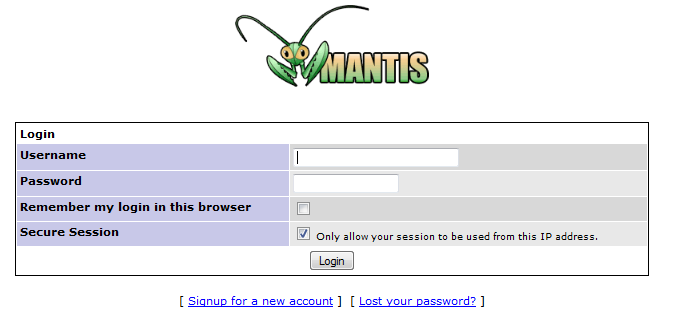
\includegraphics[scale=0.6]{./content/Immagini/mantis}
	\caption{Schermata di login di Mantis}
	\label{login_password}
\end{figure}

\subsection{Strumenti a supporto del processo di gestione del progetto}

\subsubsection{Dropbox}
\label{dropbox}
\textbf{Dropbox} è un servizio di cloud che consente di condividere directory e file tra più utenti. Verrà creata una cartella \textit{Ingegneria del Software} condivisa da tutti i membri del gruppo. La presenza del client ufficiale disponibile per la maggior parte dei sistemi operativi ha fatto cadere la scelta su questo servizio cloud.\\
Versione utilizzata: \textbf{2.4.11}

\paragraph{\underline{Installazione}:} per l'installazione dei client \textbf{Dropbox} seguire la seguente procedura:
\begin{itemize}
\item Collegarsi al sito internet \url{https://www.dropbox.com/install?os=linux}
\item Scegliere la propria distribuzione e la tipologia di architettura del proprio pc. Verrà scaricato un file con cui si potrà procedere all'installazione;
\item Installare il software seguendo la procedura;
\item Aprire il software e seguire la procedura per creare un nuovo account o per effettuare il login con le proprie credenziali.
\end{itemize}

\subsubsection{GanttProject}
\label{ganttproject}
\textbf{GanttProject} è un software Open Source per la gestione di attività di progetto. La scelta è ricaduta su tale applicativo per i seguenti motivi:
\begin{itemize}
	\item Portabilità, essendo il software scritto in Java;
	\item Open source;
	\item Permette la generazione di diagrammi di Gantt\glossario{} e delle risorse;
	\item Consente di esportare i diagrammi in formato \verb!PNG! o \verb!HTML!.
\end{itemize}
Versione utilizzata: \textbf{2.6.5}

\paragraph{\underline{Installazione}:} per l'installazione dell'applicativo, seguire la seguente procedura:
\begin{itemize}
\item Collegarsi al sito internet \url{http://www.ganttproject.biz/}
\item Selezionare \textit{Download GanttProject 2.6.5}. Verrà caricata una pagina in cui sarà presente il collegamento adatto al proprio sistema operativo;
\item Selezionare \textit{GanttProject 2.6.5}. Verrà caricata una pagina contenente le ultime versioni disponibili del software;
\item Selezionare l'ultima versione. Verrà caricata un ulteriore pagina di download;
\item Selezionare il file da scaricare. Partirà automaticamente il download del file;
\item Una volta scaricato, procedere con l'installazione.
\end{itemize}

\subsubsection{GitHub}
\label{github}
\textbf{GitHub} è un servizio web di hosting per lo sviluppo di progetti, che utilizza il controllo di versione Git\g{}. Sono stati creati due repository\g{} privati, sfruttando il servizio di \textbf{GitHub Education}\footnote{\url{https://education.github.com/}}:
\begin{itemize}
\item Documentazione: \url{https://github.com/nicolobissacco/7MonkeysDoc}
\item Codice: \url{https://github.com/nicolobissacco/7MonkeysCode}
\end{itemize}
Rendere operativi gli account dei membri del team, collegandoli ai repository\g{}, sarà compito degli \textit{Amministratori}.\\
La scelta è ricaduta su Git\g{} per i seguenti motivi:
\begin{itemize}
\item La possibilità di poter lavorare localmente, senza bisogno di essere connessi a internet;
\item Git\g{} era già stato usato da vari membri del team;
\item La possibilità di ignorare certe estensioni dei file (gitignore);
\item La presenza di innumerevoli client grafici, per chi non volesse utilizzarlo da shell.
\end{itemize}
Per i membri del gruppo, che non vogliono utilizzare la shell, sono consigliati i seguenti client:
\begin{itemize}
\item \textbf{Sourcetree:} disponibile per i sistemi Windows\g{} e Mac OS\g{};
\item \textbf{Giteye:} disponibile per  i sistemi Linux\g{}.
\end{itemize}

\paragraph{\underline{Registrazione}:} per utilizzare il servizio, è necessario registrarsi presso il portare di \textbf{GitHub}. Seguire la seguente procedura:
\begin{itemize}
\item Collegarsi al sito internet \url{https://github.com/}
\item Compilare la form e selezionare \textit{Sign up for GitHub};
\item Seguire la procedura indicata nella e-mail che viene inviata all'indirizzo indicato nella form.
\end{itemize}

\paragraph{\underline{Creazione milestone}:} per creare una nuova milestone\g{}, si segua la seguente procedura:
\begin{itemize}
\item Accedere al repository\g{}, collegandosi all'indirizzo web opportuno (vedi sez.\ref{github});
\item Selezionare \textit{Issues}. Verrà caricata una pagina contenente la lista dei ticket attualmente aperti;
\item Selezionare \textit{Milestones}. Verrà caricata una pagina contenente le milestone\g{} create;
\item Selezionare \textit{Create a new milestone}. Verrà caricata una pagina contenente una form  (vedi \ref{github_milestone});
\item Compilare i campi della form;
\item Selezionare \textit{Create milestone}.
\end{itemize}
\begin{figure}[h]
	\centering
	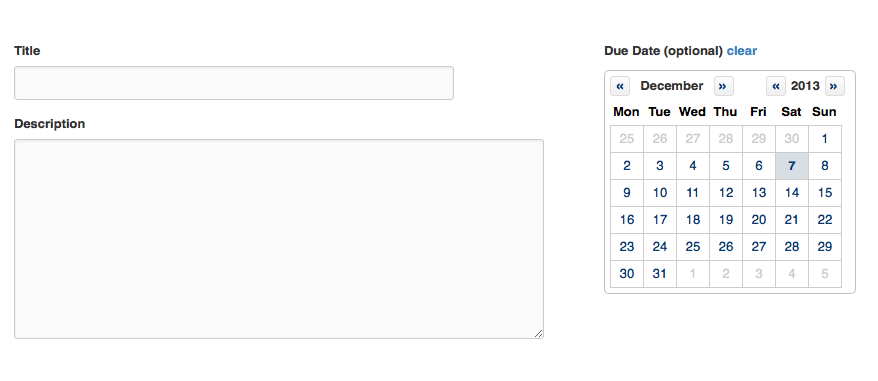
\includegraphics[scale=0.5]{./content/Immagini/Screen1}
	\caption{Interfaccia di GitHub per la creazione di una milestone}
	\label{github_milestone}
\end{figure}

\paragraph{\underline{Creazione ticket}:} per creare un nuovo ticket, si segua la seguente procedura:
\begin{itemize}
\item Accedere al repository\g{}, collegandosi all'indirizzo web opportuno (vedi sez.\ref{github});
\item Selezionare \textit{Issues}. Verrà caricata una pagina contenente la lista dei ticket attualmente aperti;
\item Selezionare \textit{New Issue}. Verrà caricata una pagina contenente una form (vedi figura \ref{newticketgithub});
\item Compilare la form assegnando: titolo, descrizione, milestone, membro destinatario del ticket ed eventuali \textit{labels};
\item Selezionare \textit{Submit new Issue}.
\end{itemize}
\begin{figure}[h!]
	\centering
	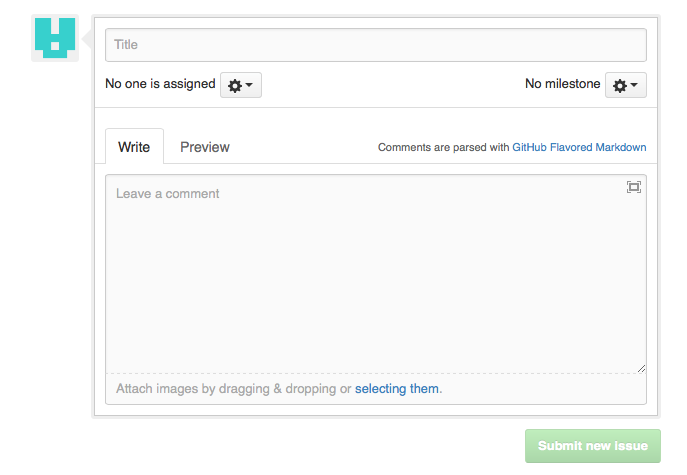
\includegraphics[scale=0.5]{./content/Immagini/Screen2}
	\caption{Interfaccia di GitHub per la creazione di un ticket.}
	\label{newticketgithub}
\end{figure}

\paragraph{\underline{Chiusura milestone}:} per chiudere la milestone\g{}, si segua la seguente procedura:
\begin{itemize}
\item Accedere al repository\g{}, collegandosi all'indirizzo web opportuno (vedi sez.\ref{github});
\item Selezionare \textit{Issues}. Verrà caricata una pagina contenente la lista dei ticket attualmente aperti;
\item Selezionare \textit{Milestones}. Verrà caricata una pagina contenente le milestone\g{} create;
\item Selezionare \textit{Close} in corrispondenza della milestone\g{} che si vuole chiudere.
\end{itemize}

\subsubsection{Google Calendar}
\label{googlecalendar}
Per sfruttare le potenzialità di questo strumento collaborativo, è stato creato un calendario condiviso tra i vari membri del gruppo denominato \textbf{GruppoSWE}. Tale servizio permette di notificare:
\begin{itemize}
\item In quali date un certo membro non è disponibile;
\item In quali date c'è una riunione o un evento rilevante ai fini del gruppo.
\end{itemize}
Grazie alla gestione delle notifiche di \textbf{Google Calendar}\g{}, è possibile far in modo che 24 ore prima di un evento rilevante venga inviata una email a tutti i membri del gruppo come promemoria.

\paragraph{\underline{Registrazione}:} per usufruire di questo servizio, è necessario possedere un account \textbf{Google}. Sarà cura degli \textit{Amministratori}, di condividere il calendario con tutti i membri del gruppo. Per ottenere un account \textbf{Google}, seguire la seguente procedura:
\begin{itemize}
\item Collegarsi al sito internet: \url{https://accounts.google.com/SignUp?hl=it}
\item Compilare la form con i propri dati;
\item Selezionare \textit{Passaggio successivo};
\item Seguire la procedura indicata nella e-mail di conferma che verrà inviata all'indirizzo precedentemente inserito.
\end{itemize}

\paragraph{\underline{Creare un nuovo evento}:} per creare un nuovo evento, seguire la seguente procedura:
\begin{itemize}
\item Collegarsi al sito internet: \url{https://www.google.com/calendar/}
\item Se necessario, effettuare l'accesso al sistema di \textbf{Google} inserendo le proprie credenziali;
\item Selezionare la freccia a fianco al nome del calendario;
\item Selezionare \textit{Crea evento in questo calendario};
\item Compilare la form con tutti i dati necessari;
\item Selezionare \textit{Salva}.
\end{itemize}

\subsubsection{Google Drive}
\label{googledrive}
Servizio di cloud storage, che permette di immagazzinare e condividere file con più persone. Viene utilizzato dal team per organizzare i file sviluppati tramite il servizio \textbf{Google Docs}\g{}. Per questo scopo è stata creata e condivisa una cartella denominata \textbf{swe}.

\paragraph{\underline{Registrazione}:} per usufruire del servizio è necessario possedere un account \textbf{Google}. Per la procedura, si veda il paragrafo \textit{Registrazione} nella sezione \ref{procedurecalendar}.

\paragraph{\underline{Creazione di un nuovo documento condiviso}:} per creare un nuovo documento condiviso e salvarlo nella cartella condivisa, seguire la seguente procedura:
\begin{itemize}
\item Collegarsi al sito internet: \url{https://drive.google.com/}
\item Se necessario, effettuare l'accesso al sistema di \textbf{Google} inserendo le proprie credenziali;
\item Selezionare \textit{Shared with Me};
\item Selezionare la cartella \textit{swe};
\item Selezionare \textit{Create} e seguire la procedura di creazione di un nuovo documento condiviso.
\end{itemize}

\subsubsection{Scripts}
\label{scripts}
Per facilitare la compilazione e il controllo dei documenti, è stato creato un \textit{Makefile} disponibile nel repository\g{} della documentazione. (vedi fig. \ref{filesystem}). Il Makefile consente di:
\begin{itemize}
\item Generare tutti i file della documentazione in formato \verb!.PDF!
\item Eseguire il controllo ortografico in tutti i file \verb!.TEX! che compongono la struttura della documentazione;
\item Eliminare i file generati dalla compilazione dei file \verb!.TEX!
\end{itemize}

\paragraph{\underline{Generare la documentazione}:} per compilare la documentazione, in occasione di una consegna di revisione, seguire la seguente procedura:
\begin{itemize}
\item Aprire il terminale;
\item Posizionarsi nella cartella \textit{Scripts} (vedi fig. \ref{filesystem});
\item Digitare \verb!make RX! con \verb!X! corrispondente alla revisione che si sta per consegnare (\verb!R! per Revisione, \verb!P! per Progettazione, \verb!Q! per Qualifica, \verb!A! per Accettazione). Verranno generati tutti i file e verranno salvati nell'apposita directory \textit{Consegne}.
\end{itemize}

\paragraph{\underline{Eseguire controllo ortografico}:} per eseguire il controllo ortografico, seguire la seguente procedura:
\begin{itemize}
\item Aprire il terminale;
\item Posizionarsi nella cartella \textit{Scripts} (vedi fig. \ref{filesystem});
\item Digitare \verb!make aspell!. Verrà avviata la procedura di controllo ortografico, utilizzando \textbf{Aspell} (vedi sez. \ref{aspell}). Il controllo verrà effettuato su tutti i file \verb!.TEX! che compongono la struttura della documentazione.
\end{itemize}

\paragraph{\underline{Pulire il filesystem}:} per eseguire la rimozione dei file di compilazione della documentazione, seguire la seguente procedura:
\begin{itemize}
\item Aprire il terminale;
\item Posizionarsi nella cartella \textit{Scripts} (vedi fig. \ref{filesystem});
\item Digitare \verb!make clean!. Verranno rimossi tutti i file di compilazione generati da \LaTeX.
\end{itemize}